\documentclass{report}
%%%%%%%%%%%%%% preamble.tex %%%%%%%%%%%%%%
\usepackage[T1]{fontenc}
\usepackage{etoolbox}
% Page Setup
\usepackage[letterpaper, tmargin=2cm, rmargin=0.5in, lmargin=0.5in, bmargin=80pt, footskip=.2in]{geometry}
\usepackage{adjustbox}
\usepackage{graphicx}
\usepackage{tikz}
\usepackage{mathrsfs}
\usepackage{mdframed}

% Create a new toggle
\newtoggle{firstsection}

% Redefine the \chapter command to reset the toggle for each new chapter
\let\oldchapter\chapter
\renewcommand{\chapter}{\toggletrue{firstsection}\oldchapter}

% Redefine the \section command to check the toggle
\let\oldsection\section
\renewcommand{\section}{
    \iftoggle{firstsection}
    {\togglefalse{firstsection}} % If it's the first section, just switch off the toggle for next sections
    {\clearpage} % If it's not the first section, start a new page
    \oldsection
}

% Abstract Design

\usepackage{lipsum}

\renewenvironment{abstract}
 {% Start of environment
  \quotation
  \small
  \noindent
  \rule{\linewidth}{.5pt} % Draw the rule to match the linewidth
  \par\smallskip
  {\centering\bfseries\abstractname\par}\medskip
 }
 {% End of environment
  \par\noindent
  \rule{\linewidth}{.5pt} % Ensure the closing rule also matches
  \endquotation
 }

% Mathematics
\usepackage{amsmath,amsfonts,amsthm,amssymb,mathtools}
\usepackage{xfrac}
\usepackage[makeroom]{cancel}
\usepackage{enumitem}
\usepackage{nameref}
\usepackage{multicol,array}
\usepackage{tikz-cd}
\usepackage{array}
\usepackage{multirow}% http://ctan.org/pkg/multirow
\usepackage{graphicx}

% Colors
\usepackage[dvipsnames]{xcolor}
\definecolor{myg}{RGB}{56, 140, 70}
\definecolor{myb}{RGB}{45, 111, 177}
\definecolor{myr}{RGB}{199, 68, 64}
% Define more colors here...
\definecolor{olive}{HTML}{6B8E23}
\definecolor{orange}{HTML}{CC5500}
\definecolor{brown}{HTML}{8B4513}
% Hyperlinks
\usepackage{bookmark}
\usepackage[colorlinks=true,linkcolor=blue,urlcolor=blue,citecolor=blue,anchorcolor=blue]{hyperref}
\usepackage{xcolor}
\hypersetup{
    colorlinks,
    linkcolor={red!50!black},
    citecolor={blue!50!black},
    urlcolor={blue!80!black}
}

% Text-related
\usepackage{blindtext}
\usepackage{fontsize}
\changefontsize[14]{14}
\setlength{\parindent}{0pt}
\linespread{1.2}

% Theorems and Definitions
\usepackage{amsthm}
\renewcommand\qedsymbol{$\blacksquare$}

% Define a new theorem style
\newtheoremstyle{mytheoremstyle}% name
  {}% Space above
  {}% Space below
  {}% Body font
  {}% Indent amount
  {\bfseries}% Theorem head font
  {.}% Punctuation after theorem head
  {.5em}% Space after theorem head
  {}% Theorem head spec (can be left empty, meaning ‘normal’)

% Apply the new theorem style to theorem-like environments
\theoremstyle{mytheoremstyle}

\newtheorem{theorem}{Theorem}[section]  
\newtheorem{definition}[theorem]{Definition} 
\newtheorem{lemma}[theorem]{Lemma}  
\newtheorem{corollary}[theorem]{Corollary}
\newtheorem{axiom}[theorem]{Axiom}
\newtheorem{example}[theorem]{Example}
\newtheorem{equiv_def}[theorem]{Equivalent Definition}

% tcolorbox Setup
\usepackage[most,many,breakable]{tcolorbox}
\tcbuselibrary{theorems}

% Define custom tcolorbox environments here...

%================================
% EXAMPLE BOX
%================================
% After you have defined the style and other theorem environments
\definecolor{myexamplebg}{RGB}{245, 245, 245} % Very light grey for background
\definecolor{myexamplefr}{RGB}{120, 120, 120} % Medium grey for frame
\definecolor{myexampleti}{RGB}{60, 60, 60}    % Darker grey for title

\newtcbtheorem[]{Example}{Example}{
    colback=myexamplebg,
    breakable,
    colframe=myexamplefr,
    coltitle=myexampleti,
    boxrule=1pt,
    sharp corners,
    detach title,
    before upper=\tcbtitle\par\vspace{-20pt}, % Reduced the space after the title
    fonttitle=\bfseries,
    description font=\mdseries,
    separator sign none,
    description delimiters={}{}, % No delimiters around the title
}{ex}
%================================
% Solution BOX
%================================
\makeatletter
\newtcolorbox{solution}{enhanced,
	breakable,
	colback=white,
	colframe=myg!80!black,
	attach boxed title to top left={yshift*=-\tcboxedtitleheight},
	title=Solution,
	boxed title size=title,
	boxed title style={%
			sharp corners,
			rounded corners=northwest,
			colback=tcbcolframe,
			boxrule=0pt,
		},
	underlay boxed title={%
			\path[fill=tcbcolframe] (title.south west)--(title.south east)
			to[out=0, in=180] ([xshift=5mm]title.east)--
			(title.center-|frame.east)
			[rounded corners=\kvtcb@arc] |-
			(frame.north) -| cycle;
		},
}
\makeatother

% %================================
% % Question BOX
% %================================
\makeatletter
\newtcbtheorem{question}{Question}{enhanced,
	breakable,
	colback=white,
	colframe=myb!80!black,
	attach boxed title to top left={yshift*=-\tcboxedtitleheight},
	fonttitle=\bfseries,
	title={#2},
	boxed title size=title,
	boxed title style={%
			sharp corners,
			rounded corners=northwest,
			colback=tcbcolframe,
			boxrule=0pt,
		},
	underlay boxed title={%
			\path[fill=tcbcolframe] (title.south west)--(title.south east)
			to[out=0, in=180] ([xshift=5mm]title.east)--
			(title.center-|frame.east)
			[rounded corners=\kvtcb@arc] |-
			(frame.north) -| cycle;
		},
	#1
}{question}
\makeatother

%%%%%%%%%%%%%%%%%%%%%%%%%%%%%%%%%%%%%%%%%%%
% TABLE OF CONTENTS
%%%%%%%%%%%%%%%%%%%%%%%%%%%%%%%%%%%%%%%%%%%


\usepackage{tikz}
\definecolor{doc}{RGB}{0,60,110}
\usepackage{titletoc}
\contentsmargin{0cm}
\titlecontents{chapter}[14pc]
{\addvspace{30pt}%
	\begin{tikzpicture}[remember picture, overlay]%
		\draw[fill=doc!60,draw=doc!60] (-7,-.1) rectangle (-0.9,.5);%
		\pgftext[left,x=-5.5cm,y=0.2cm]{\color{white}\Large\sc\bfseries Chapter\ \thecontentslabel};%
	\end{tikzpicture}\color{doc!60}\large\sc\bfseries}%
{}
{}
{\;\titlerule\;\large\sc\bfseries Page \thecontentspage
	\begin{tikzpicture}[remember picture, overlay]
		\draw[fill=doc!60,draw=doc!60] (2pt,0) rectangle (4,0.1pt);
	\end{tikzpicture}}%
\titlecontents{section}[3.7pc]
{\addvspace{2pt}}
{\contentslabel[\thecontentslabel]{3pc}}
{}
{\hfill\small \thecontentspage}
[]
\titlecontents*{subsection}[3.7pc]
{\addvspace{-1pt}\small}
{}
{}
{\ --- \small\thecontentspage}
[ \textbullet\ ][]

\makeatletter
\renewcommand{\tableofcontents}{
	\chapter*{%
	  \vspace*{-20\p@}%
	  \begin{tikzpicture}[remember picture, overlay]%
		  \pgftext[right,x=15cm,y=0.2cm]{\color{doc!60}\Huge\sc\bfseries \contentsname};%
		  \draw[fill=doc!60,draw=doc!60] (13,-.75) rectangle (20,1);%
		  \clip (13,-.75) rectangle (20,1);
		  \pgftext[right,x=15cm,y=0.2cm]{\color{white}\Huge\sc\bfseries \contentsname};%
	  \end{tikzpicture}}%
	\@starttoc{toc}}
\makeatother

\newcommand{\liff}{\llap{$\iff$}}
\newcommand{\rap}[1]{\rrap{\text{ (#1)}}}
\newcommand{\red}[1]{\textcolor{red}{#1}}
\newcommand{\blue}[1]{\textcolor{blue}{#1}}
\newcommand{\vi}[1]{\textcolor{violet}{#1}}
\newcommand{\olive}[1]{\textcolor{olive}{#1}}
\newcommand{\teal}[1]{\textcolor{teal}{#1}}
\newcommand{\brown}[1]{\textcolor{brown}{#1}}
\newcommand{\orange}[1]{\textcolor{orange}{#1}}
\newcommand{\tCaC}{\text{ \CaC }}
\newcommand{\CaC}{\red{CaC} }
\newcommand{\As}[1]{Assume \red{#1}}
\newcommand{\vdone}{\vi{\text{ (done) }}}
\newcommand{\bdone}{\blue{\text{ (done) }}}
\newcommand{\tdone}{\teal{\text{ (done) }}}
\newcommand{\odone}{\olive{\text{ (done) }}}
\newcommand{\bodone}{\brown{\text{ (done) }}}
\newcommand{\ordone}{\orange{\text{ (done) }}}
\newcommand{\ld}{\lambda}
\newcommand{\vecta}[1]{\textbf{#1}}
\newcommand{\set}[1]{\left\{ #1 \right\}}
\newcommand{\bset}[1]{\Big\{ #1 \Big\}}
\newcommand{\inR}{\in\R}
\newcommand{\inn}{\in\N}
\newcommand{\inz}{\in\Z}
\newcommand{\inr}{\in\R}
\newcommand{\inc}{\in\C}
\newcommand{\inq}{\in\Q}
\newcommand{\norm}[1]{\| #1 \|}
\newcommand{\bnorm}[1]{\Big\| #1 \Big\|}
\newcommand{\gen}[1]{\langle #1 \rangle}
\newcommand{\abso}[1]{\left|#1\right|}
\newcommand{\myref}[2]{\hyperref[#2]{#1\ \ref*{#2}}}
\newcommand{\customref}[2]{\hyperref[#1]{#2}}
\newcommand{\power}[1]{\mathcal{P}(#1)}
\newcommand{\dcup}{\mathbin{\dot{\cup}}}
\newcommand{\diam}[1]{\text{diam}\, #1}
\newcommand{\at}{\Big|}
\newcommand{\quotient}{\diagup}
\let\originalphi\phi % Store the original \phi in \originalphi
\renewcommand{\phi}{\varphi} % Redefine \phi to \varphi
\newcommand{\pfi}{\originalphi} % Define \pfi to display the original \phi
\newcommand{\diota}{\dot{\iota}}
\newcommand{\Log}{\operatorname{Log}}
\newcommand{\id}{\text{\textbf{id}}}
\usepackage{amsmath}

\makeatletter
\NewDocumentCommand{\extp}{e{^}}{%
  \mathop{\mathpalette\extp@{#1}}\nolimits
}
\NewDocumentCommand{\extp@}{mm}{%
  \bigwedge\nolimits\IfValueT{#2}{^{\extp@@{#1}#2}}%
  \IfValueT{#1}{\kern-2\scriptspace\nonscript\kern2\scriptspace}%
}
\newcommand{\extp@@}[1]{%
  \mkern
    \ifx#1\displaystyle-1.8\else
    \ifx#1\textstyle-1\else
    \ifx#1\scriptstyle-1\else
    -0.5\fi\fi\fi
  \thinmuskip
}
\makeatletter
\usepackage{pifont}
\makeatletter
\newcommand\Pimathsymbol[3][\mathord]{%
  #1{\@Pimathsymbol{#2}{#3}}}
\def\@Pimathsymbol#1#2{\mathchoice
  {\@Pim@thsymbol{#1}{#2}\tf@size}
  {\@Pim@thsymbol{#1}{#2}\tf@size}
  {\@Pim@thsymbol{#1}{#2}\sf@size}
  {\@Pim@thsymbol{#1}{#2}\ssf@size}}
\def\@Pim@thsymbol#1#2#3{%
  \mbox{\fontsize{#3}{#3}\Pisymbol{#1}{#2}}}
\makeatother
% the next two lines are needed to avoid LaTeX substituting upright from another font
\input{utxmia.fd}
\DeclareFontShape{U}{txmia}{m}{n}{<->ssub * txmia/m/it}{}
% you may also want
\DeclareFontShape{U}{txmia}{bx}{n}{<->ssub * txmia/bx/it}{}
% just in case
%\DeclareFontShape{U}{txmia}{l}{n}{<->ssub * txmia/l/it}{}
%\DeclareFontShape{U}{txmia}{b}{n}{<->ssub * txmia/b/it}{}
% plus info from Alan Munn at https://tex.stackexchange.com/questions/290165/how-do-i-get-a-nicer-lambda?noredirect=1#comment702120_290165
\newcommand{\pilambdaup}{\Pimathsymbol[\mathord]{txmia}{21}}
\renewcommand{\lambda}{\pilambdaup}
\renewcommand{\tilde}{\widetilde}
\DeclareMathOperator*{\esssup}{ess\,sup}
\newcommand{\bluecheck}{}%
\DeclareRobustCommand{\bluecheck}{%
  \tikz\fill[scale=0.4, color=blue]
  (0,.35) -- (.25,0) -- (1,.7) -- (.25,.15) -- cycle;%
}


\usepackage{tikz}
\newcommand*{\DashedArrow}[1][]{\mathbin{\tikz [baseline=-0.25ex,-latex, dashed,#1] \draw [#1] (0pt,0.5ex) -- (1.3em,0.5ex);}}

\newcommand{\C}{\mathbb{C}}	
\newcommand{\F}{\mathbb{F}}
\newcommand{\N}{\mathbb{N}}
\newcommand{\Q}{\mathbb{Q}}
\newcommand{\R}{\mathbb{R}}
\newcommand{\Z}{\mathbb{Z}}



\title{\Huge{NCKU 112.2}\\
Geometry 1}
\author{\huge{Eric Liu}}
\date{}
\begin{document}
\maketitle
\newpage% or \cleardoublepage
% \pdfbookmark[<level>]{<title>}{<dest>}
\pdfbookmark[section]{\contentsname}{toc}
\tableofcontents
\pagebreak
\chapter{HW}
\section{HW1}
\begin{mdframed}
  In this section, by a \textbf{curve} in $\R^n$, we mean a function form an open interval $I$ to $\R^n$.  We say a curve is \textbf{differentiable} if it is infinitely differentiable (smooth). That is, $\gamma ^{(n)}(t)$ exists for all $n\inn$ and for all $t \in I$. Clearly, for each differentiable curve $\gamma $, the function $\gamma^{(n)}:I\rightarrow \R$ (also a curve) must be continuous.  We say a differentiable curve $\gamma  :I\rightarrow \R^n$ is \textbf{regular} if $\gamma '(t)\neq 0$ for all $t  \in I$. We say a differentiable curve $\gamma :I\rightarrow \R^n$ is a \textbf{parametrized by arc-length} if $\abso{\gamma '(t)}=1$ for all $t \in I$.\\
\end{mdframed}
\begin{mdframed}

\end{mdframed}
\begin{mdframed}
\textbf{Trick to parametrize by arc-length}.\\

Given a regular curve $\gamma :I\rightarrow \R^n$ and fix $t_0 \in I$. We use
\begin{align*}
  s(t)=\int_{t_0}^t \abso{\gamma  ' (x)}dx
\end{align*}
to define the arc-length of  $\gamma $ from $\gamma (t_0)$ to $\gamma (t)$. Because $\gamma $ is regular, by FTC, it is clear that $s$ is one-to-one.\\

Let $t(s)$ be the inverse of $s$. Define 
 \begin{align*}
\beta (s)\triangleq \alpha (t(s))
\end{align*}
We have by Chain rule 
\begin{align*}
\beta '(s)&=t'(s)\alpha '(t(s))\\
&=\frac{\alpha '(t(s))}{s'(t)}\\
&=\frac{\alpha '(t(s))}{\abso{\alpha '(t(s))}}
\end{align*}
Now, $\beta $ is clearly a regular curve, and 
\begin{align*}
\int_{0}^x \abso{\beta '(s)}ds=x
\end{align*}
\end{mdframed} 
\begin{mdframed}
Now, suppose a curve $\gamma(s) $ is parametrized by arc-length. We see that for all $s \in I$ 
\begin{align*}
\frac{d}{ds} (\gamma '\cdot \gamma ')(s)=2(\gamma ''\cdot \gamma ')(s)
\end{align*}
Then because $\gamma '$ is constant $1$, this implies for all $s$ 
\begin{align}
\label{6}
\gamma ''(s) \perp \gamma '(s)
\end{align}
This let us naturally define the \textbf{curvature} $\kappa$ of $\gamma $ by 
\begin{align*}
\kappa (s)=\abso{\gamma ''(s)}
\end{align*}
It is clear that if $\gamma $ is linear (a straight line), then the curvature $\kappa(s)$ is $0$ for all $s$. 
\end{mdframed}
\begin{mdframed}
For a regular curve $\gamma $, we define its \textbf{unit tangent} by 
\begin{align*}
T(t)=\frac{\gamma '(t)}{\abso{\gamma '(t)}}
\end{align*}
and we define its \textbf{unit normal} by 
\begin{align*}
N(t)=\frac{T'(t)}{\abso{T'(t)}}
\end{align*}
and define its \textbf{binormal} vector by 
\begin{align*}
B(t)=T(t) \times N(t)
\end{align*}
Notice that we have $T(t)\perp N(t)$ from \myref{Equation}{6}. Fix $t_0$. We say 
\begin{align*}
\set{T(t),N(t),B(t)}\text{ form a \textbf{positively oriented orthonormal basis} of $\R^3$ }
\end{align*}
This basis in general is constantly changing, yet always form an orthonormal basis.\\

In a geoemtric sense, we shall note that the curve $\gamma :I\rightarrow \R^3$ stay on a plane if and only if $B$ is a constant (does not change orientation).\\

In the same spirit, $T'$ measure how curved a curve is.  (Notice that $\abso{T'}$ generally is not a constant unlike $\abso{T}$ and $\abso{N}$ ). Again, in the same spirit, $B'$ measure how fast $\gamma $ leave the plane (osculating plane) spanned by $T$ and $N$. 
\end{mdframed}
\begin{mdframed}
Given two vectors $u,v \inr^n$, we use  \textbf{dot product} 
\begin{align*}
u\cdot v= u_1v_1+\cdots + u_nv_n
\end{align*}
to denote the Euclidean inner product, and we use \textbf{length} 
\begin{align*}
\abso{u}=\sqrt{\sum_{k=1}^n u_k^2} 
\end{align*}
to denote the Euclidean norm. Note that we clearly have 
\begin{align*}
\abso{u}=\sqrt{u\cdot u} 
\end{align*}
\end{mdframed}
\begin{theorem}
\textbf{(Differentiate the Dot Product)} Given two parametrized curves $u,v:(a,b)\rightarrow \R^n$, such that $u,v$ are differentiable at  $t \in (a,b)$. We have 
\begin{align*}
\frac{d}{dt}\big(u(t)\cdot v(t) \big)= u'(t)\cdot v(t)+u(t)\cdot v'(t)
\end{align*}
\end{theorem}
\begin{proof}
\begin{align*}
\frac{d}{dt}\big(u(t)\cdot v(t) \big)&=\frac{d}{dt}\sum_{k=1}^n u_k(t)v_k(t)\\
&=\sum_{k=1}^n \frac{d}{dt} u_k(t)v_k(t)\\
&=\sum_{k=1}^n u_k'(t)v_k(t)+u_k(t)v_k'(t)\\
&=\sum_{k=1}^n u_k'(t)v_k(t)+\sum_{k=1}^n u_k(t)v_k'(t)\\
&=u'(t)\cdot v(t)+u(t)\cdot v'(t)
\end{align*}
\end{proof}
\begin{mdframed}
For the result above, sometimes we write 
\begin{align*}
  (u\cdot v)'=u'\cdot v+ u \cdot v'
\end{align*}
\end{mdframed}
\begin{question}{1-2: 2}{}

Let \(\alpha(t)\) be a parametrized curve which does not pass through the origin. If \(\alpha(t_0)\) is the point of the trace of \(\alpha\) closest to the origin and \(\alpha'(t_0) \neq 0\), show that the position vector \(\alpha(t_0)\) is orthogonal to \(\alpha'(t_0)\).
\end{question}
\begin{proof}
Define $g:I\rightarrow \R$ by 
\begin{align*}
g(t)\triangleq \abso{\alpha (t)}^2=(\alpha \cdot \alpha )(t)
\end{align*}
Notice that 
\begin{align*}
g'(t)=(2\alpha '\cdot \alpha )(t)\text{ if exists }
\end{align*}
From premise, we know $g$ attains minimum at $t_0$. This tell us 
\begin{align*}
0=g'(t_0)=(2\alpha '\cdot \alpha )(t_0)
\end{align*}
Then, we can deduce 
\begin{align*}
\alpha '(t_0)\cdot \alpha (t_0)=0
\end{align*}
This implies $\alpha (t_0)\perp \alpha '(t_0)$. 
\end{proof}
\begin{question}{1-2: 5}{}

Let \(\alpha : I \rightarrow \mathbb{R}^3\) be a parametrized curve, with \(\alpha''(t) \neq 0\) for all \(t \in I\). Show that \(|\alpha(t)|\) is a nonzero constant if and only if \(\alpha(t)\) is orthogonal to \(\alpha'(t)\) for all \(t \in I\).
\end{question}
\begin{proof}
We wish to prove 
\begin{align*}
\exists \beta  \inr^*,  \forall t \in I, \abso{\alpha (t)}=\beta  \iff \forall t \in I , (\alpha \cdot \alpha ')(t)=0
\end{align*}
Define $g:I\rightarrow \R$ by 
\begin{align*}
g(t)\triangleq \abso{\alpha (t)}^2=(\alpha \cdot \alpha )(t)
\end{align*}

Notice that 
\begin{align}
\label{1.2.5.1}
g'(t)=(2\alpha '\cdot \alpha )(t)
\end{align}
$(\longrightarrow)$\\

From premise, $g$ is a constant on  $I$. This implies  $g'(t)=0$  for all $t \in I$. Then, from \myref{Equation}{1.2.5.1}, we see 
\begin{align*}
  (\alpha \cdot \alpha ')(t)=0\text{ for all $t \in I$ }
\end{align*}
$(\longleftarrow)$\\

Again, from  \myref{Equation}{1.2.5.1}, we deduce 
\begin{align*}
\forall t \in I , (\alpha \cdot \alpha ')(t)=0 \implies \forall t \in I, g'(t)=0
\end{align*}

This implies $g$ is a constant, which implies $\abso{\alpha }$ is a constant, that is 
\begin{align*}
\exists \beta \inr, \abso{\alpha (t)}=\beta 
\end{align*}
Lastly, we have to show 
\begin{align*}
\vi{\text{ $\beta \neq 0$ }}
\end{align*}
\As{$\beta =0$}. Then, we see $\alpha (t)=0$ for all $t \in I$. This implies $\alpha ''(t)=0 $ for all $t \in I$, which \CaC to the premise. $\vdone$
\end{proof}
\begin{question}{1-3:2}{}
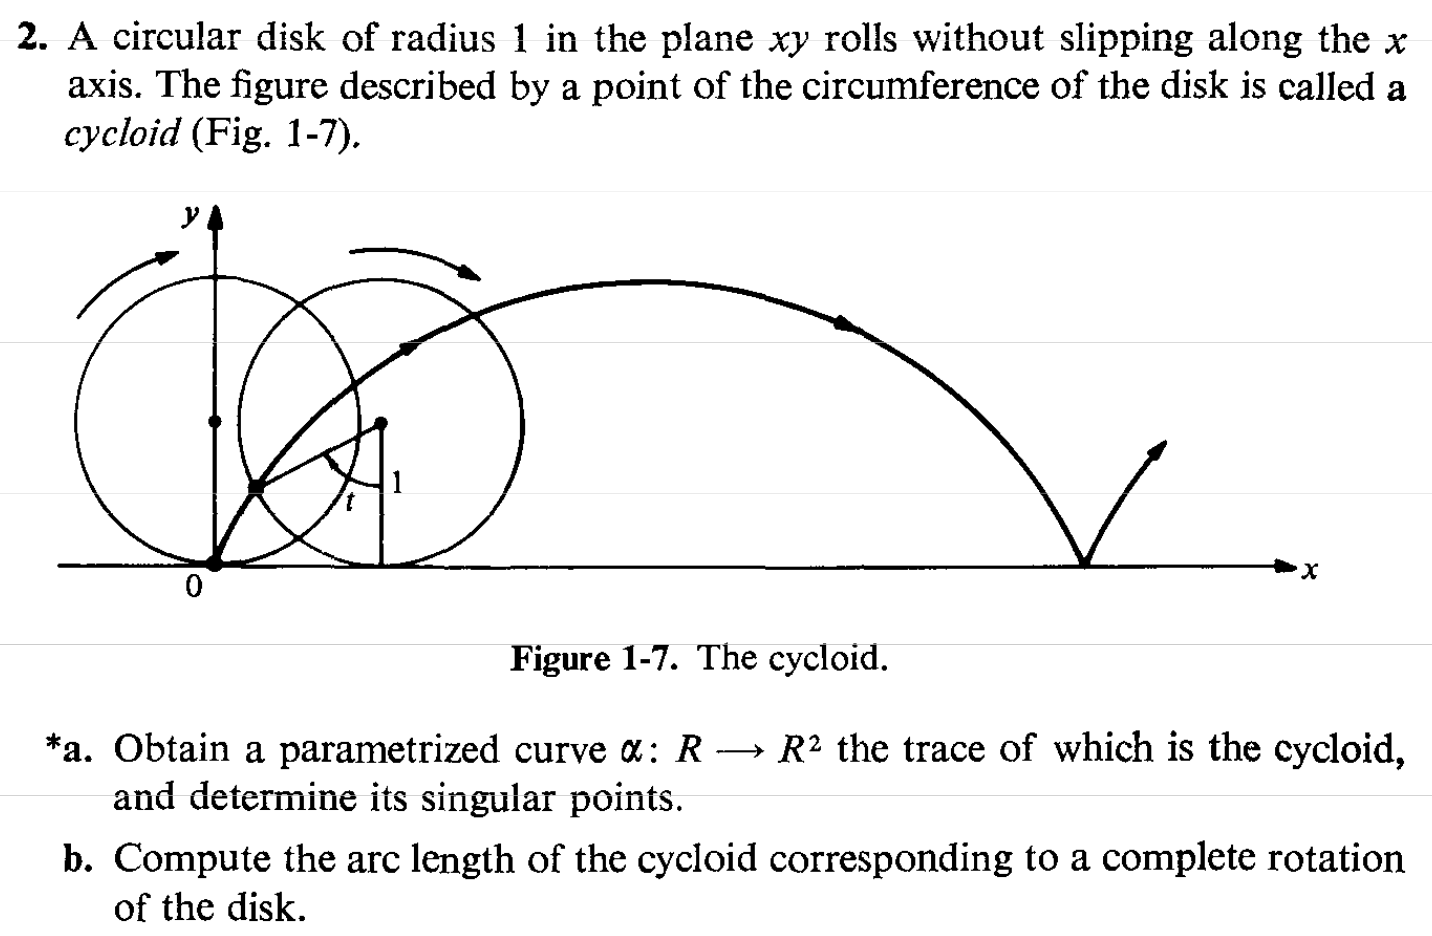
\includegraphics[height=10cm,width=18cm]{1.png}
\end{question}
\begin{proof}
The solution of the question \textbf{a} is 
\begin{align*}
\alpha (t)=(t-\sin t,1-\cos t)
\end{align*}
Compute 
\begin{align*}
\alpha'(t)=(1-\cos t,\sin t)
\end{align*}
and compute
\begin{align*}
\abso{\alpha '(t)}=\sqrt{1-2\cos t +\cos^2 t +\sin^2 t}  = \sqrt{2}\cdot \sqrt{1-\cos t}  
\end{align*}
This implies the singular points are 
\begin{align*}
  \set{2n\pi : n\inz}
\end{align*}


The solution of the question \textbf{b} is then 
\begin{align*}
\int_0^{2\pi} \abso{\alpha '(t)}dt&=\sqrt{2}\int_0^{2\pi} \sqrt{1-\cos t}dt \\
&=\sqrt{2} \int_{0}^{2\pi} \sqrt{2} \abso{\sin \frac{t}{2}}dt  \\
&=2\int_0^{2\pi}\abso{\sin \frac{t}{2}}dt\\
&=4 \int_{0}^{\pi}\sin (\frac{t}{2})dt\\
&=-8 \cos \frac{t}{2}\Big|_0^{\pi}
\end{align*}

\end{proof}
\begin{question}{1-3:4}{}
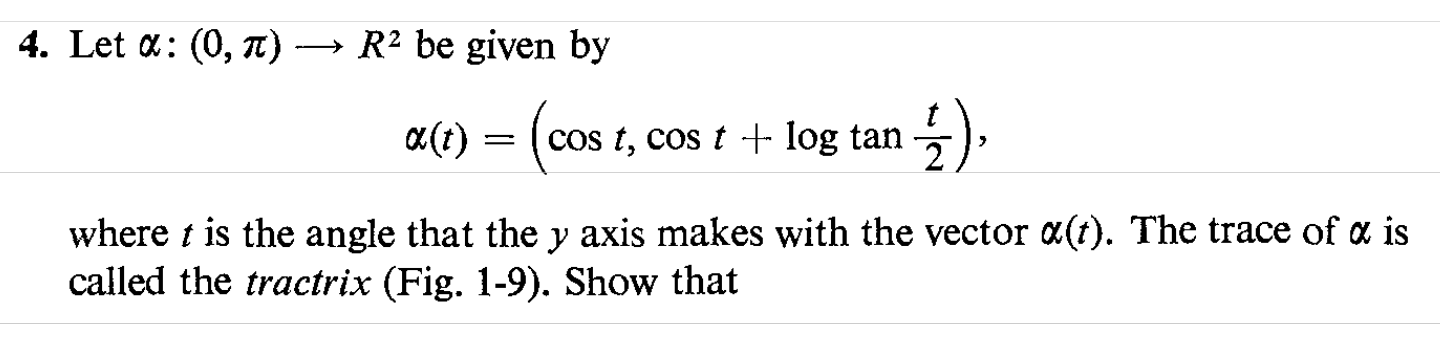
\includegraphics[height=4cm,width=18cm]{3.png}
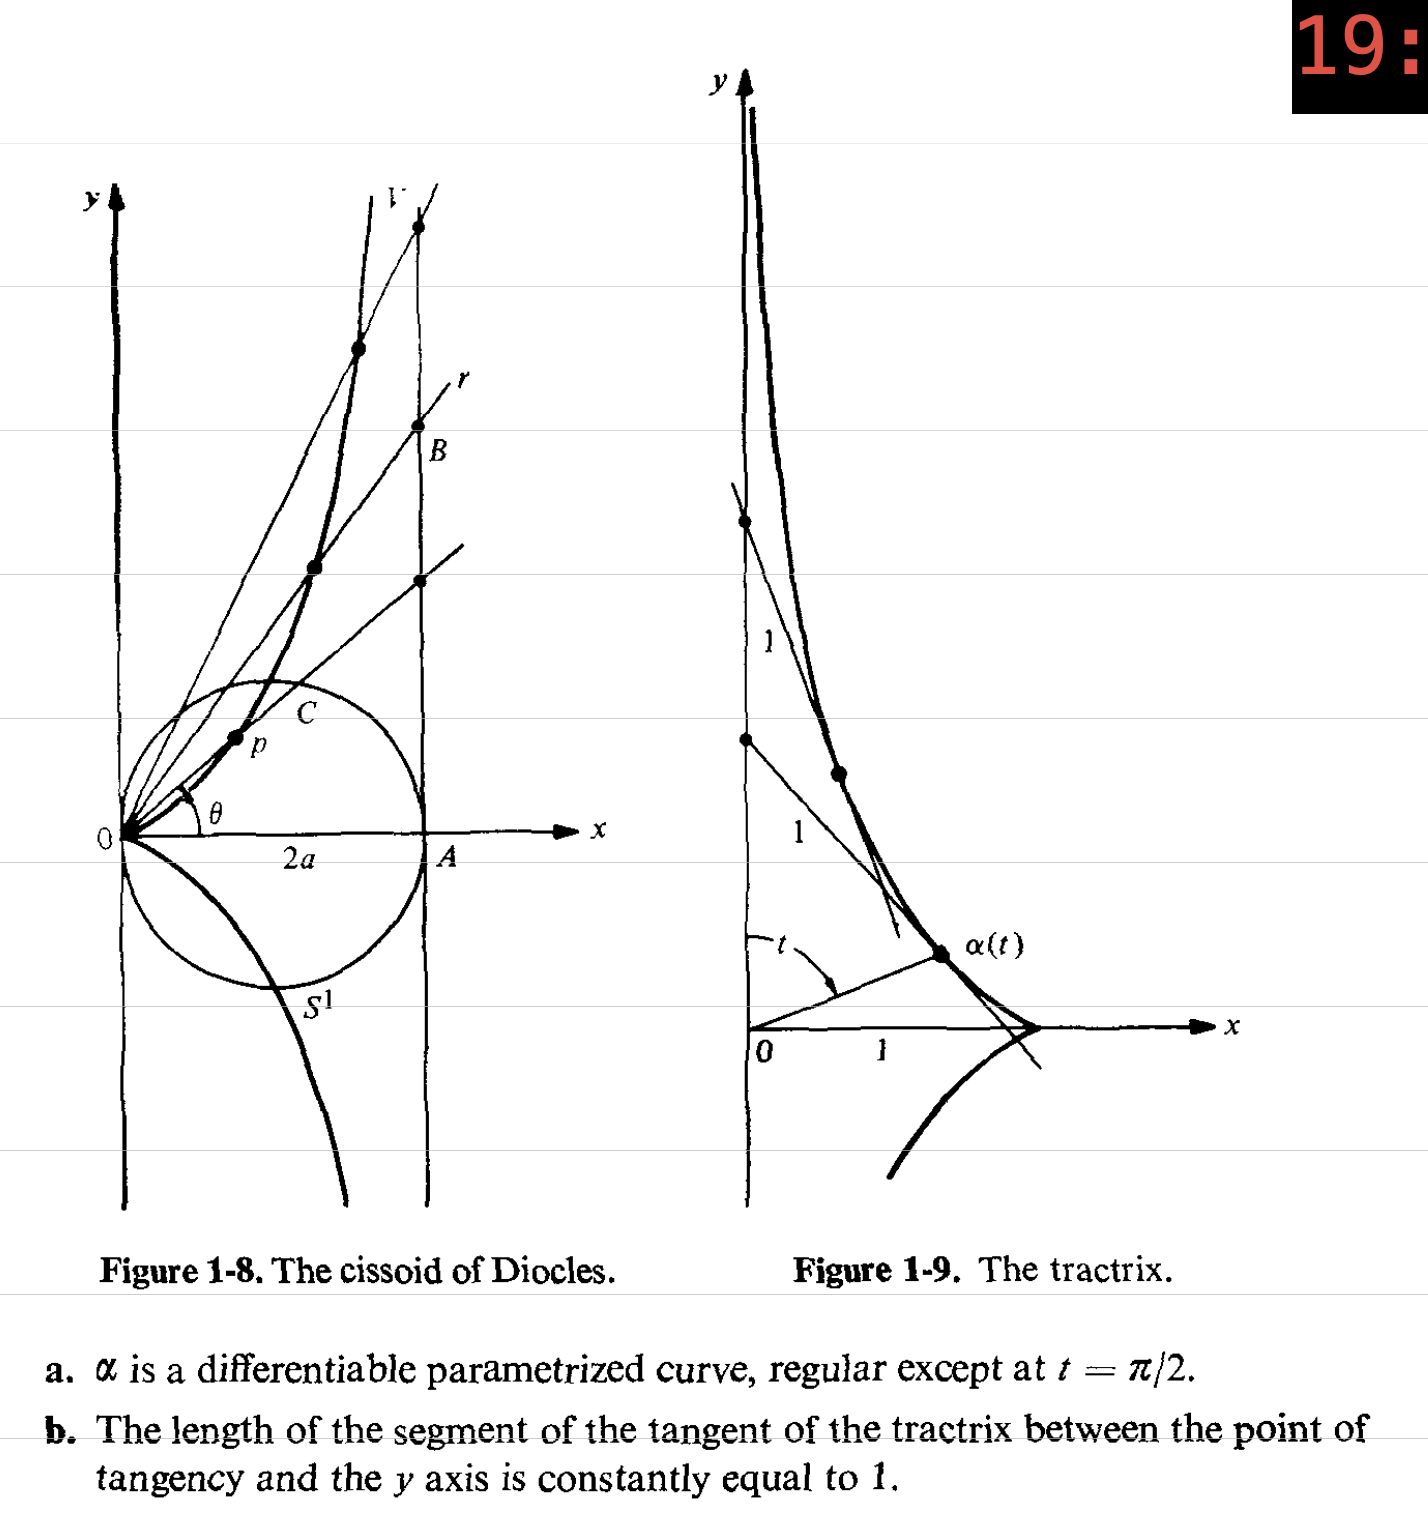
\includegraphics[height=18cm,width=18cm]{2.png}
Typo correction: $\alpha (t)=(\sin t,\cos t + \ln \tan \frac{t}{2})$
\end{question}
\begin{proof}
\textbf{(a)}

Notice that the interval $I$ is  $(0,\pi)$. It is clear that 
\begin{enumerate}[label=(\alph*)]
  \item $\sin t$ is smooth on $\R$
  \item $\cos t$ is smooth on $\R$
  \item $\ln t$ is smooth on $\R$
  $\tan \frac{t}{2}$ is smooth on $I$
\end{enumerate}
Then it follows that $\alpha $ is a differentiable curve.\\

Compute 
\begin{align*}
\alpha '(t)=(\cos t,- \sin t + \frac{1}{\tan \frac{t}{2}} \cdot \sec^2 \frac{t}{2}\cdot \frac{1}{2})
\end{align*}
Because $\cos t=\alpha '_1(t)$ is $0$ on  $I$ only when  $t=\frac{\pi}{2}$, we know $\alpha $ is regular on $I$ except possibly at  $t=\frac{\pi}{2}$.\\

Compute 
\begin{align*}
\alpha '(\frac{\pi}{2})=(0,-1+\frac{1}{1}\cdot 2 \cdot \frac{1}{2} )=(0,0)
\end{align*}
We now conclude $\alpha $ is regular on $I$ except  $\frac{\pi}{2}$. \\

\textbf{(b)}

A useful Identity give us 
\begin{align*}
\alpha '(t)=(\cos t,-\sin t+ \csc t)
\end{align*}
From the following facts
\begin{enumerate}[label=(\alph*)]
  \item the first argument of the segment is from $0$ to  $\sin t =\alpha (t)$
  \item $\alpha_x'(t)=\cos t$
  \item $\frac{\sin t}{\cos t}=\tan t$
\end{enumerate}
We conclude that the length of the segment is 
\begin{align*}
\abso{\tan t}\cdot \abso{\alpha '(t)}&= \abso{\tan t} \cdot \sqrt{\cos ^2 t + \sin^2 t - 2 \sin t \csc t + \csc ^2 t }\\
&=\abso{\tan t} \cdot \sqrt{1-2+\csc ^2 t}\\
&=\abso{\tan t } \cdot \sqrt{\csc ^2 t-1}=\abso{\tan t } \cdot  \sqrt{\cot ^2 t} =1
\end{align*}



\end{proof}
\begin{question}{}{}
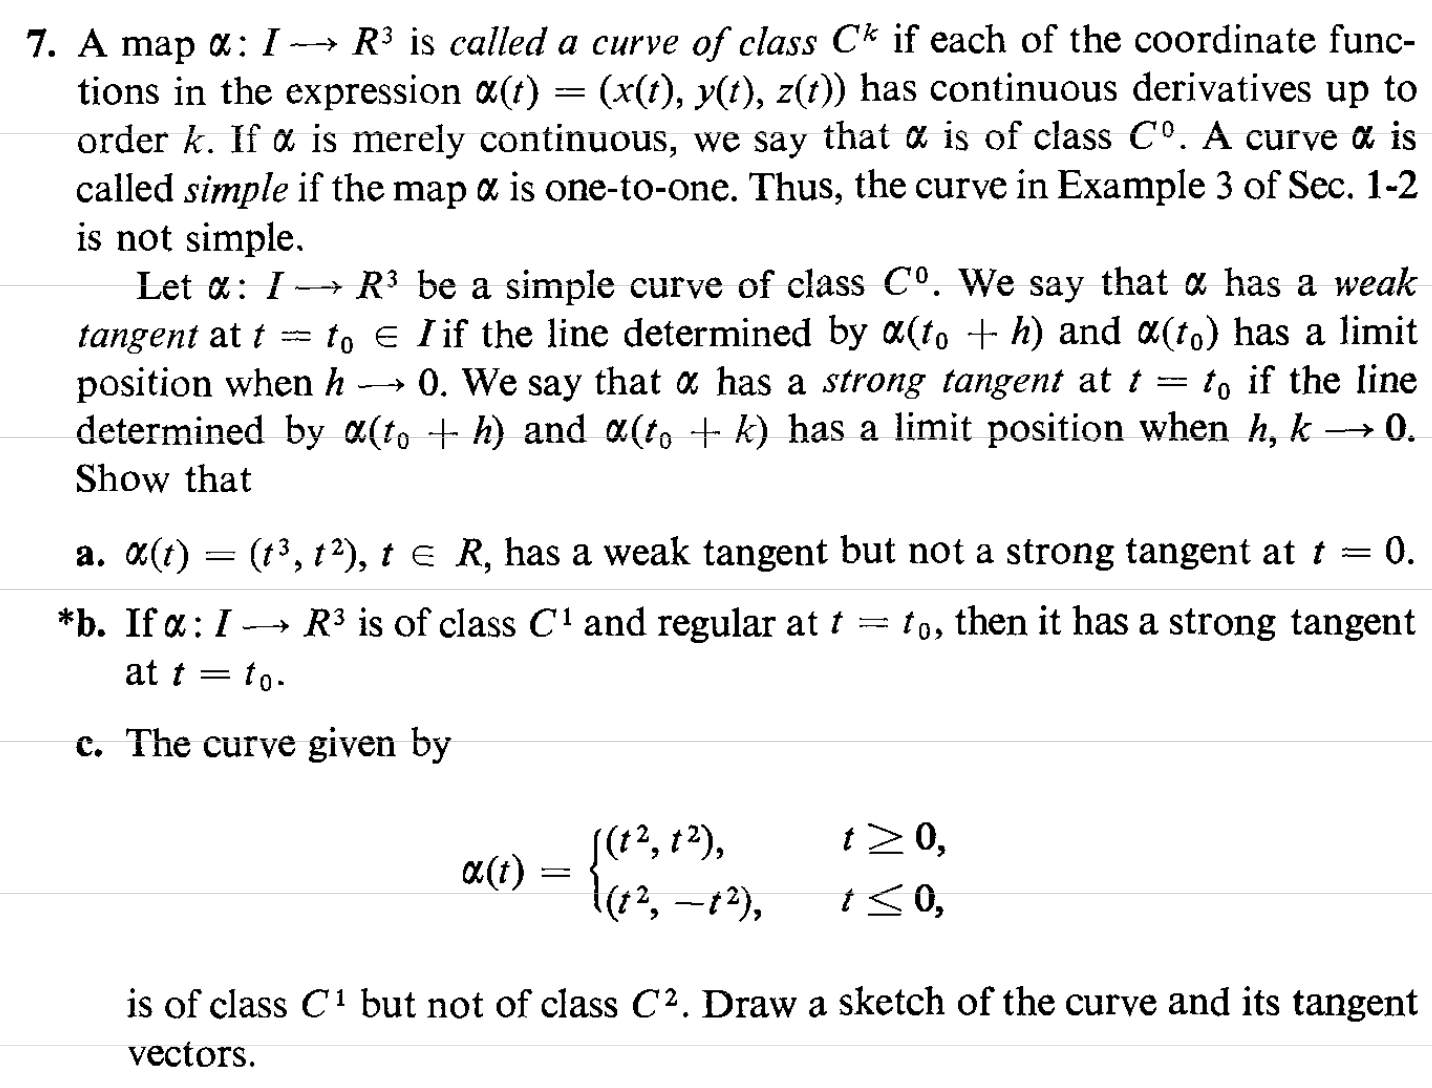
\includegraphics[height=14cm,width=18cm]{qu4}
\end{question}
\begin{proof}
\textbf{(a)}
\begin{align*}
\frac{\alpha (t)}{t}\to (0,0)\text{ as $t \to 0^-$ }
\end{align*}
\begin{align*}
\frac{\alpha (h)-\alpha (k)}{h-k}=\frac{\Big(h^3-k^3 ,h^2-k^2\Big)}{h-k}=\Big(h^2+hk+k^2 , h+k \Big) \to 
\end{align*}
\textbf{(b)} 
By MVT, for each $h,k$ there exists a set of real numbers $\set{c_x,c_y,c_z}$ between $t+h$ and  $t+k$ such that 
 \begin{align*}
\frac{\alpha (t_0+h)-\alpha  (t_0+k)}{h-k}=\Big(x'(c_x),y'(c_y),z'(c_z) \Big)
\end{align*}
Then because 
\begin{align*}
h,k  \to 0 \implies t_0+h ,t_0+k \to t_0 \implies c_x,c_y,c_z \to t_0
\end{align*}
Then from the fact $\alpha $ is of class $C^1$ ($x',y',z'$ are all continuous), we can now deduce 
\begin{align*}
\frac{\alpha (t_0+h)-\alpha (t_0+k)}{h-k}\to \alpha '(t_0)\text{ as $h,k \to 0$ }
\end{align*}
Now, because $\alpha '(t_0)\neq 0$ as $\alpha $ is regular, we see 
\begin{align*}
\lim_{h,k\to 0}\frac{\alpha (t_0+h)-\alpha (t_0+k)}{h-k}\cdot \alpha '(t_0)= \abso{\alpha '(t_0)}^2
\end{align*}
\textbf{(c)}\\

From 
\begin{align*}
\alpha (t)=\Big(t^2,\begin{cases}
  t^2& \text{ if $t\geq 0$ }\\
  -t^2& \text{ if $t\leq 0$ }
\end{cases} \Big)
\end{align*}
Compute 
\begin{align*}
\alpha '(t)=\Big(2t,\begin{cases}
  2t& \text{ if $t\geq 0$ }\\
  -2t& \text{ if $t\leq 0$ }
\end{cases} \Big)
\end{align*}
Notice that the derivative at $t=0$ is computed from definition instead of product rule.\\


Now, it is clear that $x',y'$ are continuous. This implies $\alpha  \in C^1$. Yet, we see $y'$ is not differentiable at  $t=0$. This implies  $\alpha \not \in C^2$.\\

The sketch: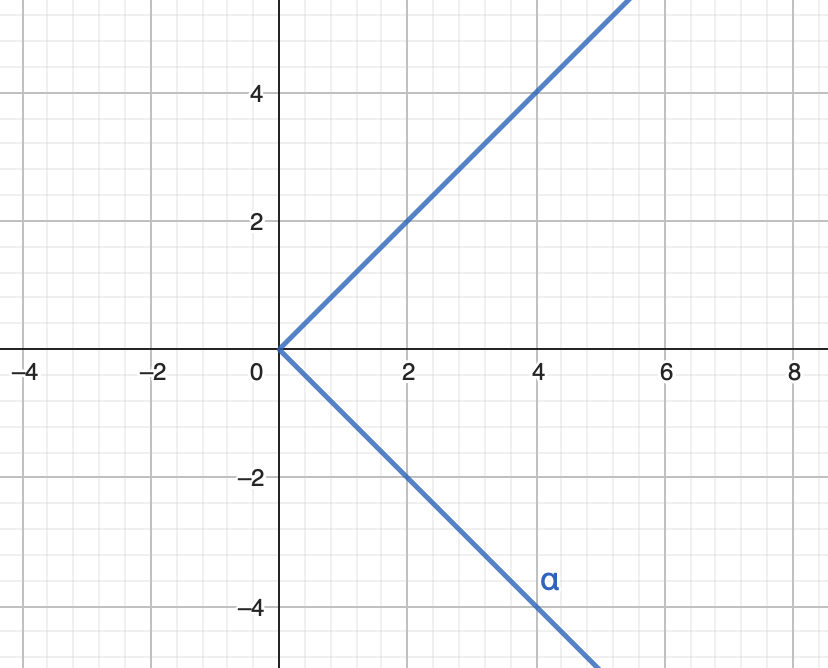
\includegraphics[height=8cm,width=15cm]{qsp}
\end{proof}
\begin{theorem}
\textbf{(MVT for curve)} Given a curve $\alpha  : [a,b]\rightarrow \R^n$ such that 
\begin{enumerate}[label=(\alph*)]
  \item $\alpha  $ is differentaible on $(a,b)$ 
  \item $\alpha  $ is continuous on $[a,b]$
\end{enumerate}
there exists $ \xi  \in (a,b)$ such that 
\begin{align*}
\abso{\alpha  (b)-\alpha  (a)}\leq \abso{\alpha  '(\xi  )}(b-a)
\end{align*}
\end{theorem}
\begin{proof}
Define $\phi:[a,b]\rightarrow \R$ by 
\begin{align*}
\phi(t)=\alpha (t)\cdot \big(\alpha (b)-\alpha (a) \big) 
\end{align*}
Clearly $\phi$ satisfy the hypothesis of Lagrange's MVT, then we know there exists $\xi \in (a,b)$ such that 
\begin{align*}
\phi(b)-\phi (a)=\phi'(\xi )\cdot (b-a)
\end{align*}
Written the equation in $\alpha $, we have 
\begin{align*}
\abso{\alpha (b)-\alpha (a)}^2= (b-a)\alpha '(\xi)\cdot \big(\alpha (b)-\alpha (a) \big)
\end{align*}
Notice that Cauchy-Schwarz inequality give us 
\begin{align*}
  (b-a)\abso{\alpha '(\xi)}\cdot \abso{\alpha (b)-\alpha (a)}&\geq (b-a)\abso{\alpha ' (\xi)\cdot \big(\alpha (b)-\alpha (a) \big)} \\
  &=\abso{\alpha (b)-\alpha (a)}^2
\end{align*}
This then implies 
\begin{align*}
  (b-a)\abso{\alpha '(\xi)}\geq \abso{\alpha (b)-\alpha (a)}
\end{align*}
\end{proof}
\begin{corollary}
\label{MVI}
\textbf{(Mean Value Inequality)} Given a curve $\alpha :[a,b]\rightarrow \R^n$ such that 
\begin{enumerate}[label=(\alph*)]
  \item $\alpha $ is differentiable on $(a,b)$ 
  \item $\alpha $ is continuous on $[a,b]$
\end{enumerate}
we have 
\begin{align*}
\abso{\alpha (b)-\alpha (a)}\leq (b-a)\sup_{(a,b)}\abso{\alpha '}
\end{align*}
\end{corollary}
\begin{question}{}{}
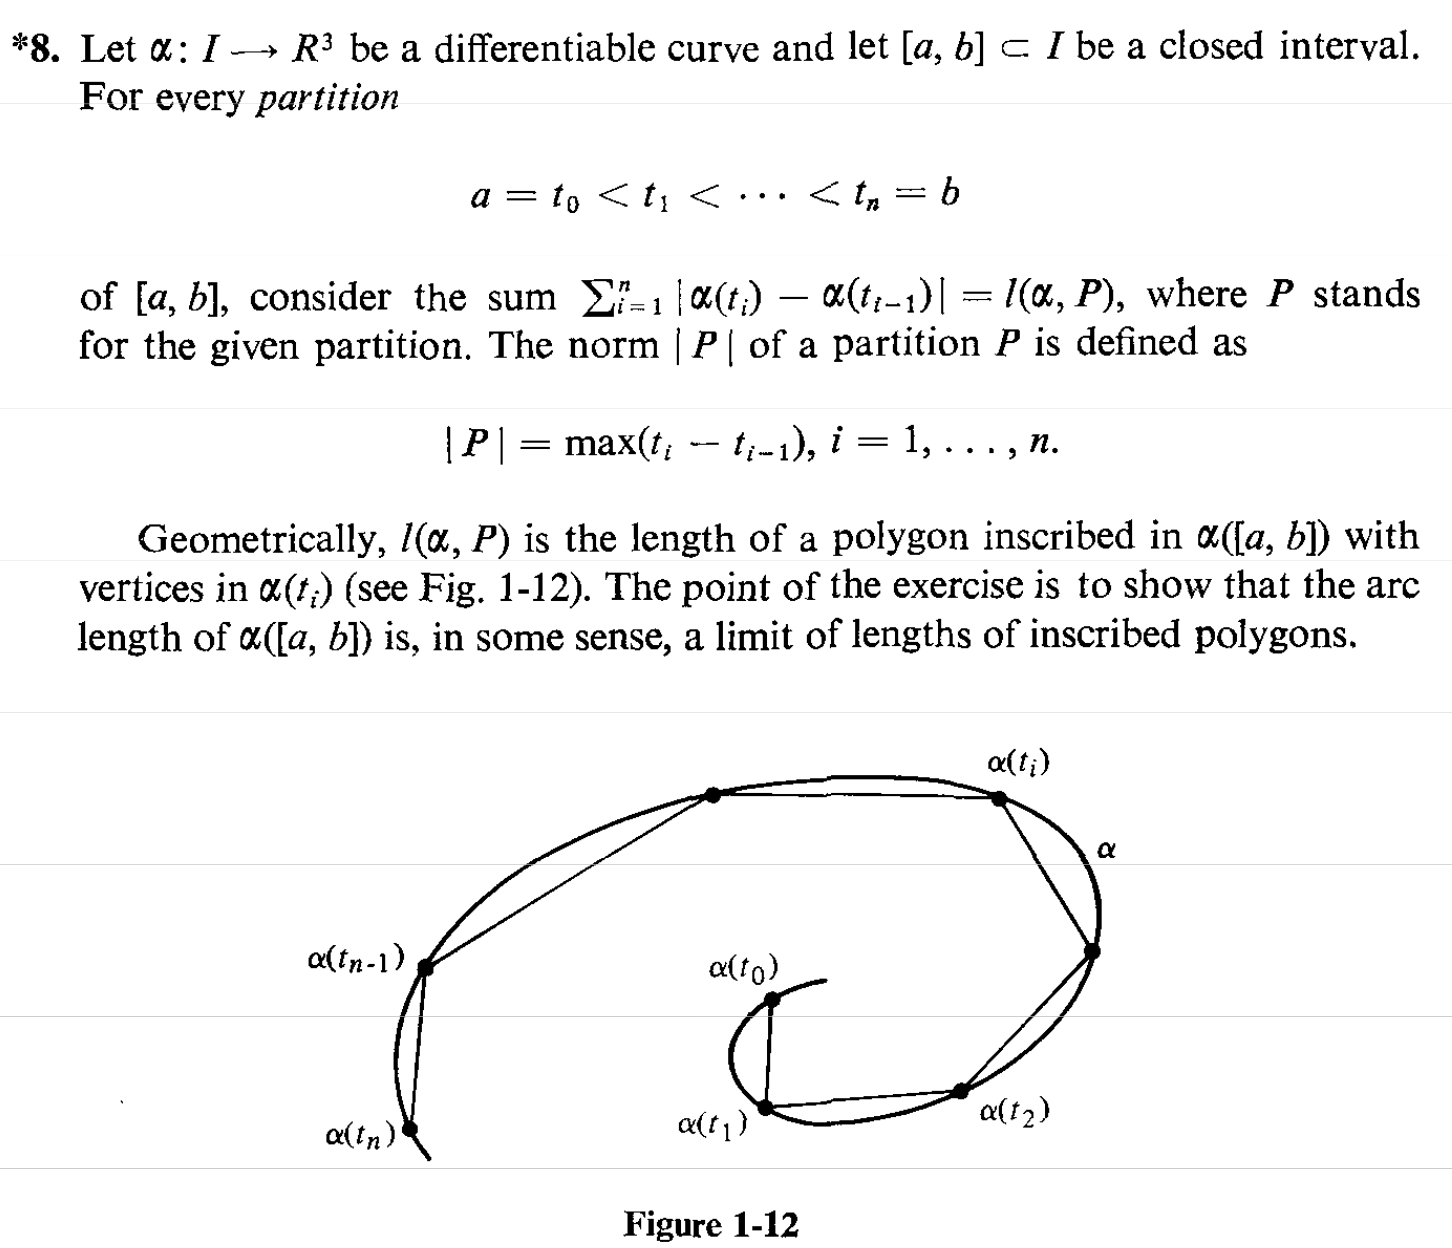
\includegraphics[height=15cm,width=18cm]{qu8}
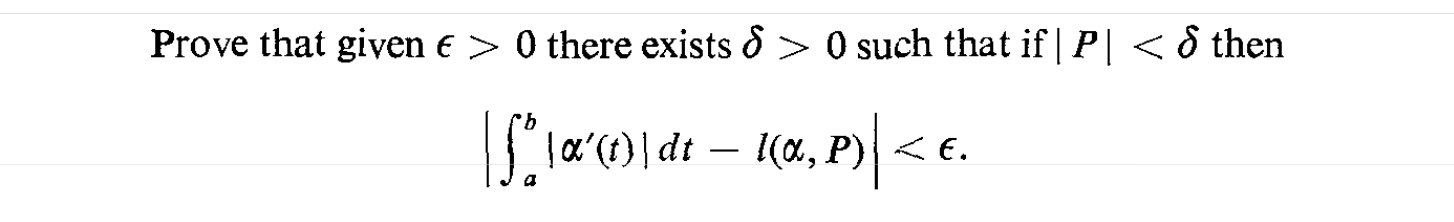
\includegraphics[height=3cm,width=18cm]{qu7}
\end{question}
\begin{proof}
We first prove 
\begin{align*}
\vi{\int_a^b \abso{\alpha '(t)}dt \geq  l(\alpha ,P)}
\end{align*}
By FTC, we have
\begin{align*}
  \abso{\alpha (t_i)-\alpha (t_{i-1})}&=\abso{\int_{t_{i-1}}^{t_i} \alpha '(t)dt}\\
&\leq \int_{t_{i-1}}^{t_i} \abso{\alpha '(t)}dt 
\end{align*}
This then implies 
\begin{align*}
l(\alpha ,P)=\sum \abso{\alpha (t_i)-\alpha (t_{i-1})}\leq \sum \int_{t_{i-1}}^{t_i}\abso{\alpha '(t)}dt=\int_a^b \abso{\alpha '(t)}dt \vdone
\end{align*}
We have reduced the problem into 
\begin{align*}
\blue{\text{ finding $\delta$ such that }\forall P: \abso{P}<\delta , \int_a^b \abso{\alpha '(t)}dt - l(\alpha ,P)<\epsilon }
\end{align*}


Because $\alpha '$ is uniformly continuous on $[a,b]$ ($\because$ continuous function on compact domain is uniformly continuous), we know there exists $\delta ' $ such that 
\begin{align*}
\abso{\alpha '(s)-\alpha '(t)}< \frac{\epsilon }{2(b-a)}\text{ if $\abso{s-t}<\delta'$ }
\end{align*}
We claim 
\begin{align*}
\blue{\text{ such $\delta'$ works }}
\end{align*}
Let $\abso{P}<\delta$, and let $s_i \in [t_{i-1},t_i]$. Because $\abso{s_i-t_i}<\delta$, we have
\begin{align}
\label{siti}
\abso{\alpha '(s_i)-\alpha '(t_i)}<\frac{\epsilon}{2(b-a)}
\end{align}
This give us 
\begin{align*}
\abso{\alpha '(s_i)}<\abso{\alpha '(t_i)} + \frac{\epsilon}{2(b-a)}
\end{align*}
Now, we can deduce 
\begin{align*}
  \int_{t_{i-1}}^{t_i} \abso{\alpha '(s)}ds&\leq   \abso{\alpha '(t_i)}\Delta t_i+ \frac{\epsilon }{2(b-a)}\Delta t_i\\
  &=\int_{t_{i-1}}^{t_i}\abso{\alpha '(t_i)}dt + \frac{\epsilon}{2(b-a)}\Delta t_i\\
 &=\abso{\int_{t_{i-1}}^{t_i} \alpha '(t_i)dt}+ \frac{\epsilon }{2(b-a)}\Delta t_i\\
  &=\abso{\int_{t_{i-1}}^{t_i} \alpha' (t_i)-\alpha '(t)dt + \int_{t_{i-1}}^{t_i} \alpha '(t)dt }+ \frac{\epsilon}{2(b-a)}\Delta t_i \\
  &\leq  \abso{\int_{t_{i-1}}^{t_i} \alpha '(t_i)-\alpha' (t)dt}+ \abso{\int_{t_{i-1}}^{t_i} \alpha '(t)dt}+\frac{\epsilon}{2(b-a)}\Delta t_i \\
  &\leq \frac{\epsilon}{2(b-a)}\Delta t_i + \abso{\alpha (t_i)-\alpha (t_{i-1})}+\frac{\epsilon}{2(b-a)}\Delta t_i\\
  &=\abso{\alpha (t_i)-\alpha (t_{i-1})}+ \frac{\epsilon }{b-a}\Delta t_i
\end{align*}
Notice that the last inequality follows from \myref{Equation}{siti}. The long deduction above then give us 
\begin{align*}
  \int_{a}^b \abso{\alpha '(t)}dt&\leq \sum \abso{\alpha (t_i)-\alpha (t_{i-1})}+ \frac{\epsilon}{b-a} (b-a)\\
&=l(\alpha ,P)+\epsilon 
\end{align*}
Then we have 
\begin{align*}
\int_a^b \abso{\alpha '(t)}dt -l(\alpha ,P)\leq \epsilon \bdone
\end{align*}
\end{proof}
\begin{question}{}{}
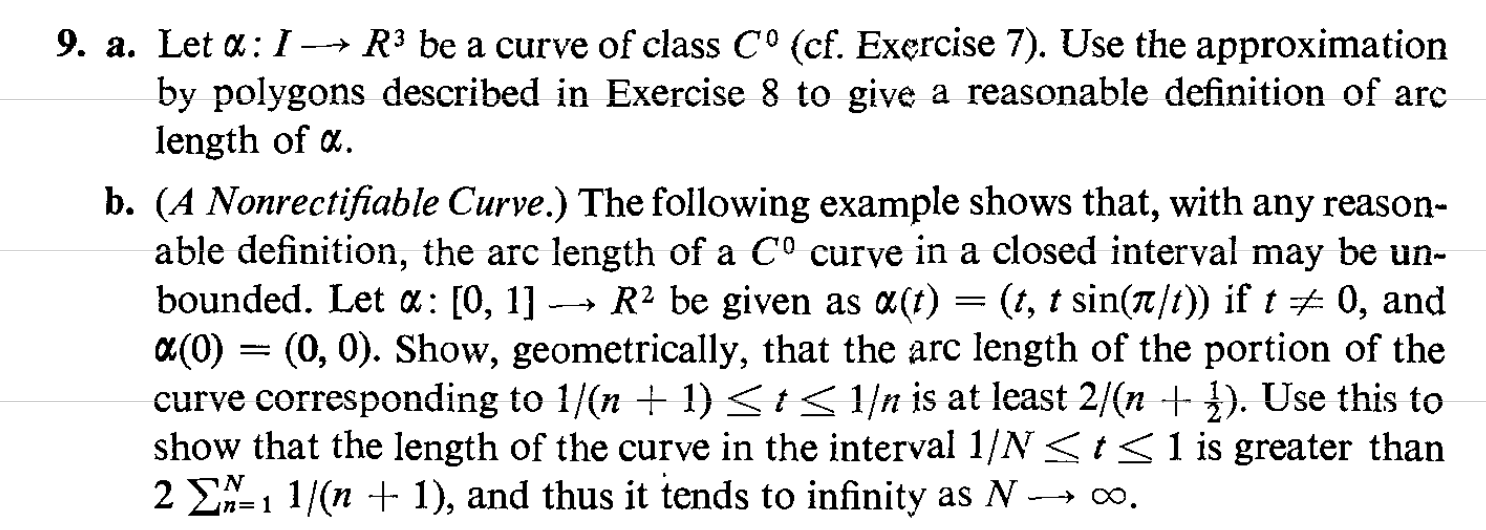
\includegraphics[height=7cm,width=18cm]{qu6}
\end{question}
\begin{proof}
\textbf{(a)} 
Suppose $I=[a,b]$. Define arc length by 
\begin{align*}
\sup_{P} l(P,\alpha )\text{ where $\sup $ runs over all partition $P$ of $[a,b]$  }
\end{align*}

\textbf{(b)}\\

Geometrically, we know the arc length of the portion of the curve corresponding to $t \in [\frac{1}{n+1},\frac{1}{n}]$ must be greater than 
\begin{align*}
\abso{\alpha \big(\frac{1}{n}\big)-\alpha \big(\frac{1}{n+\frac{1}{2}}\big)}+\abso{\alpha \big(\frac{1}{n+1} \big)-\alpha \big(\frac{1}{n+\frac{1}{2}} \big)}
\end{align*}
This 



\end{proof}
\begin{question}{}{}
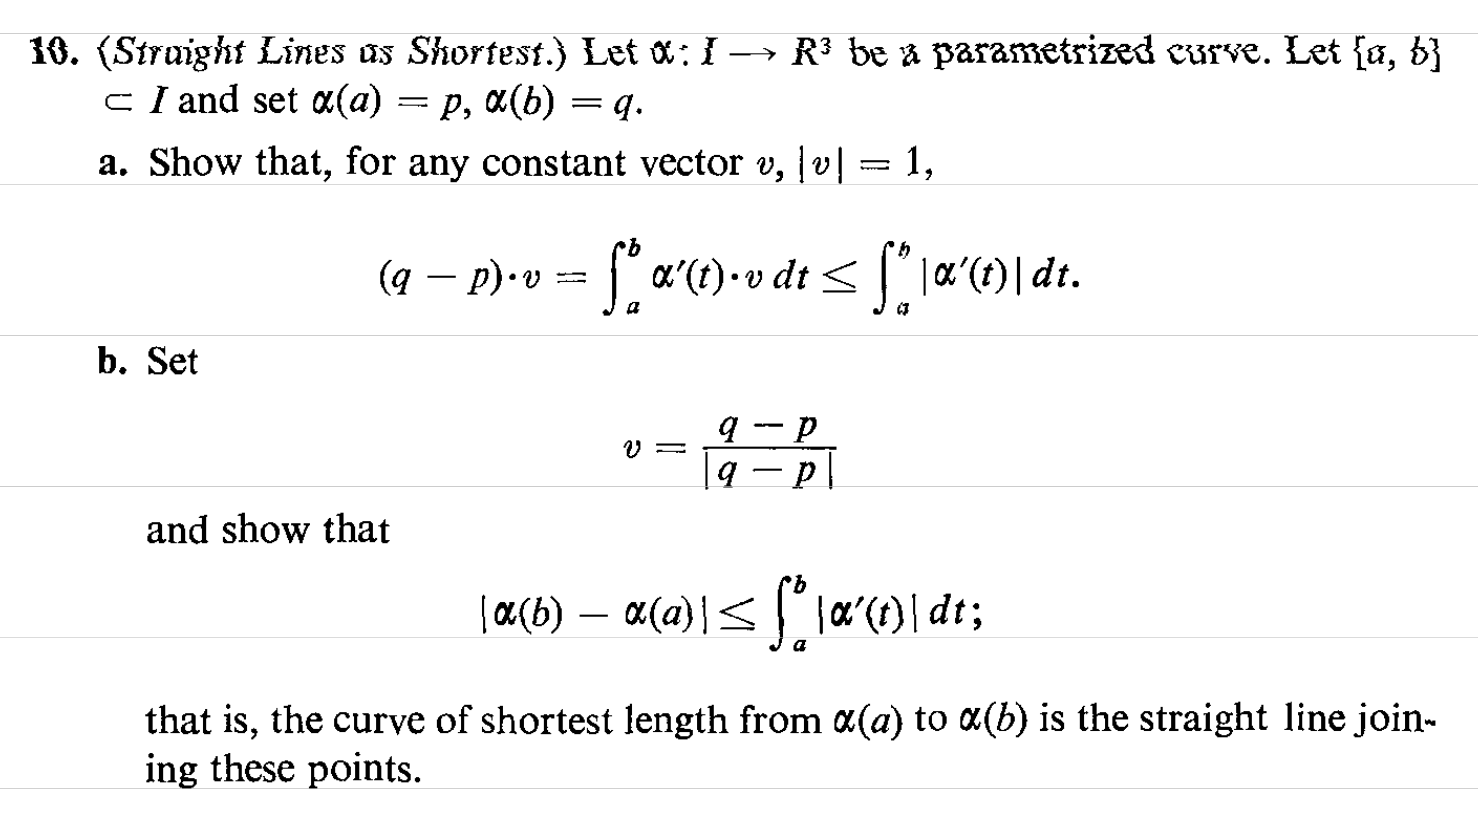
\includegraphics[height=10cm,width=18cm]{qu5}
\end{question}



\end{document}
